\chapter{Results}
\label{capitulo5}




\begin{figure}[H]
\centering
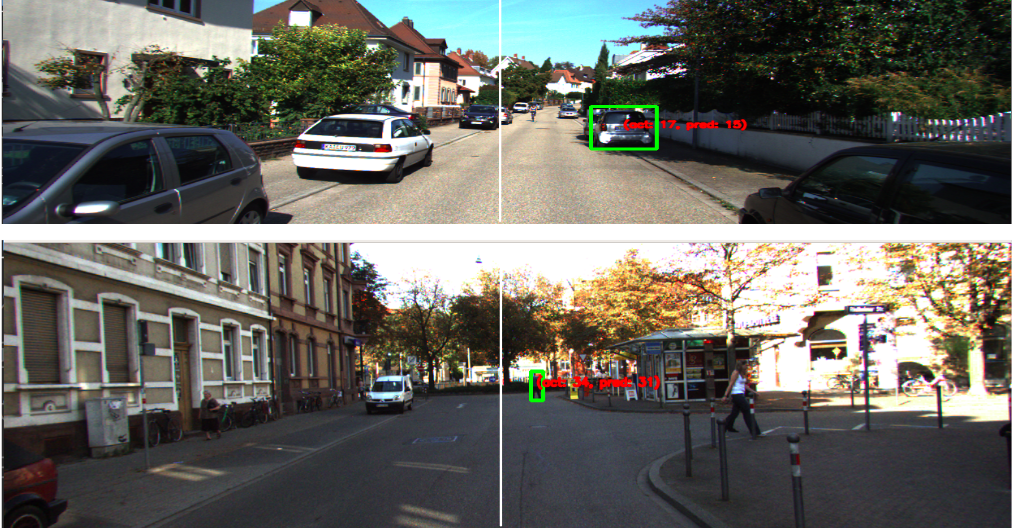
\includegraphics[width=\textwidth]{imagens/ouput.png}
\caption{Output results from framework using single stereo camera}
\label{fig:output}
\end{figure}


\section{Validation}

For validation purpose, it was used a commercial laser measurement as shown in Figure \ref{fig:laser_meas}, this model is known as Bosch DLE 40 Professional $^{\tiny{\textregistered}}$. 



\begin{figure}[H]
\centering
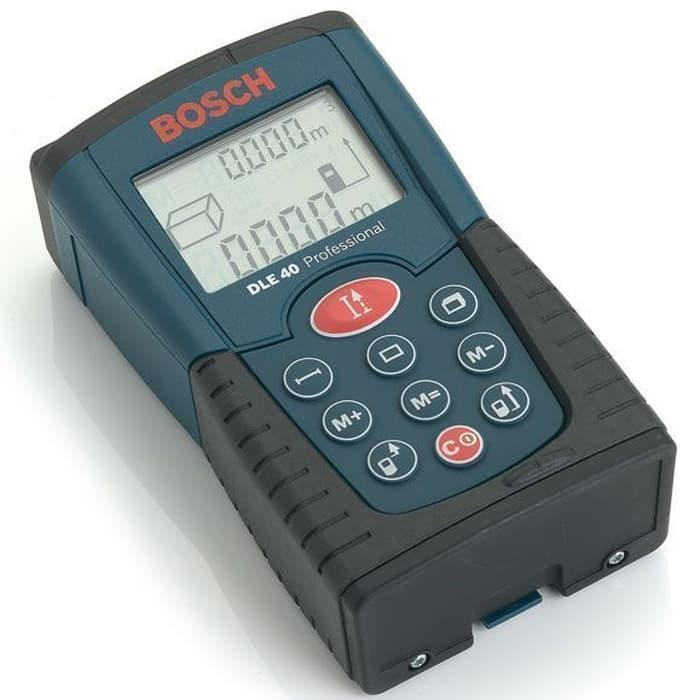
\includegraphics[scale=0.3]{imagens/trena.jpg}
\caption{Commercial laser measurer}
\label{fig:output}
\end{figure}

The instrumental error rate is $\pm 1.5 mm$, thereby we repeated the measure three times and computed the mean, and standard deviation as well. In Table \ref{tab:tab_measure} is shown the measurements with the camera positioned at $2.01$ m from the ground. And in the Figure \ref{fig:park} is shown the position of the cars along the parking lot. 



\begin{table}[H]
\centering
\caption{Measurements collected with a commercial measurer}
\begin{tabular}{l|l|l|l} 
\toprule
Car & First measure & Second measure & Third measure  \\
\#1   & 4.25          & 4.47           & 4.51           \\
\#2   & 11.01         & 11.21          & 11.11          \\
\#3   & 16.12         & 16.35          & 16.26          \\
\#4   & 19.63         & 19.69          & 19.66          \\
\#5   & 23.08         & 23.18          & 23.01          \\
\bottomrule
\end{tabular}
\label{tab:tab_measure}
\end{table} 



\begin{figure}[H]
\centering
\label{fig:park}
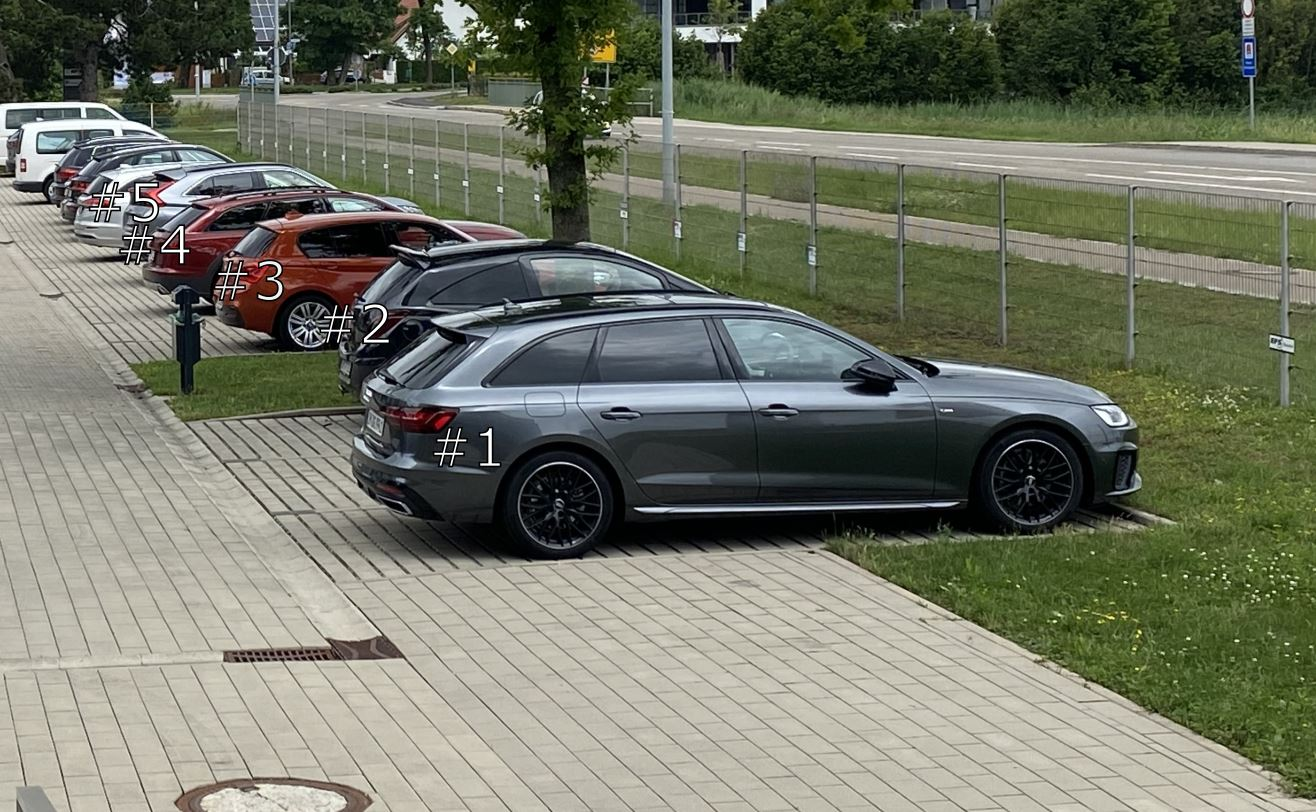
\includegraphics[scale=0.5]{imagens/park.JPG}
\caption{Position of the cars on the parking lot}
\label{fig:output}
\end{figure}
